% \documentclass{IEEEtran}
\documentclass{article}
\usepackage[utf8]{vietnam}
\usepackage{tabularx}
\usepackage{geometry}
\usepackage{longtable}
\usepackage{blindtext}
\usepackage{graphicx}
\usepackage[sorting=nyt]{biblatex}
\geometry{
  paper=a4paper,
  left=3cm,
  right=2cm,
  vmargin=2cm,
  includeheadfoot=true,
  headheight=30pt
}
\addbibresource{references.bib}
\begin{document}
% \title{\large{ \textbf{MỘT KHUÔN KHỔ HỖ TRỢ LỰA CHỌN DỊCH VỤ CỦA CÁC NHÀ CUNG CẤP ĐIỆN TOÁN ĐÁM MÂY DỰA TRÊN ĐIỂM CHUẨN CẤU HÌNH MÁY ẢO}} \\[10pt] 
% \normalsize{A SUPPORTING FRAMEWORK FOR SERVICE SELECTION OF CLOUD PROVIDER \\  BY VIRTUAL MACHINE ‘S SPEC BENCHMARK}}

% \author{\IEEEauthorblockN{Son Nguyen-Hong\IEEEauthorrefmark{1}} \\
% \IEEEauthorblockA{University of Information Technology - Vietnam National University HoChiMinh City \\
% sonnh.17@grad.uit.edu.vn}}


% \maketitle

\textbf{TÊN ĐỀ TÀI:MỘT KHUÔN KHỔ HỖ TRỢ LỰA CHỌN DỊCH VỤ CỦA CÁC NHÀ CUNG CẤP ĐIỆN TOÁN ĐÁM MÂY DỰA TRÊN ĐIỂM CHUẨN CẤU HÌNH MÁY ẢO} \\

\textbf{TÊN ĐỀ TÀI TIẾNG ANH: A SUPPORTING FRAMEWORK FOR SERVICE SELECTION OF CLOUD PROVIDER BY VIRTUAL MACHINE ‘S SPEC BENCHMARK} \\

\textbf{TÓM TẮT}: Trong giai đoạn phát triển mạnh mẽ của điện toán đám mây, việc lựa chọn dịch vụ và nhà cung cấp phù hợp là một thách thức đáng kể. Số lượng nhà cung cấp rất lớn, mỗi nhà cung cấp lại cung cấp nhiều dịch vụ với mức giá và cam kết chất lượng khác nhau. Những cam kết này phức tạp và thường không dễ kiểm chứng, vì công cụ theo dõi hiệu suất thường được thiết kế bởi từng nhà cung cấp. Do đó, việc lựa chọn đòi hỏi sự hiểu biết cao về lĩnh vực này hoặc việc thuê những chuyên gia từ nhà cung cấp. Điều này đã làm giảm sự đơn giản và tiết kiệm mà điện toán đám mây mang lại. \\

Từ nhu cầu đó, CloudBench được phát triển như một công cụ hỗ trợ người dùng trong việc lựa chọn dịch vụ từ các nhà cung cấp điện toán đám mây. CloudBench sử dụng terraform API để tự động tạo các máy ảo Linux trên các nền tảng như AWS và GCP. Đồng thời, nó sử dụng các công cụ như Passmark, FIO, Iozone và Speedtest để đo lường hiệu suất của CPU, bộ nhớ, disk và network. Các thông số thu thập từ các máy chủ được hiển thị một cách trực quan thông qua Grafana. Người dùng có thể truy cập vào trang web để xem biểu đồ và bảng thống kê, đánh giá tổng quan, so sánh hiệu năng và giá cả của các nhà cung cấp điện toán đám mây, từ đó đáp ứng được yêu cầu kỹ thuật của họ. \\

\textbf{GIỚI THIỆU}: Khái niệm về điện toán đám mây lần đầu được đưa ra bởi Jonh McCarthy: “Một ngày nào đó máy tính có thể được tổ chức và cung cấp như một tiện ích công cộng như dịch vụ điện thoại hay vận chuyển"\cite{garfinkel1999architects}. Một trong những công ty đầu tiên bắt đầu hiện thực hóa ý tưởng điện toán đám mây là Salesforce. Công ty này cung cấp dịch vụ quản lý quan hệ khách hàng dưới dạng SaaS\footnotemark \footnotetext{Software as a service}. Từ đó tới nay, rất nhiều công ty lớn như Amazon, Google, Microsoft đã tham gia vào sân chơi này, tạo ra rất nhiều sản phẩm dịch vụ để đáp ứng nhu cầu ngày càng tăng của thị trường. Song hành với đó, số lượng dịch vụ có thể sử dụng càng ngày càng lớn. Chỉ riêng ba nhà cung cấp lớn nhất là Amazon, Google, Microsoft đã lên tới hơn 600 dịch vụ \cite{amazon2023whatis,googlecloud2023product,Azure2023WhatisAzure}. Mỗi dịch vụ trong đó lại bao gồm nhiều loại với những sự lựa chọn đa dạng. Một \textit{"ma trận"} các lựa chọn đòi hỏi lượng kiến thức hoặc kinh phí lớn để đi đến quyết định đúng đắn.
\begin{figure}[h!]
  \centering
  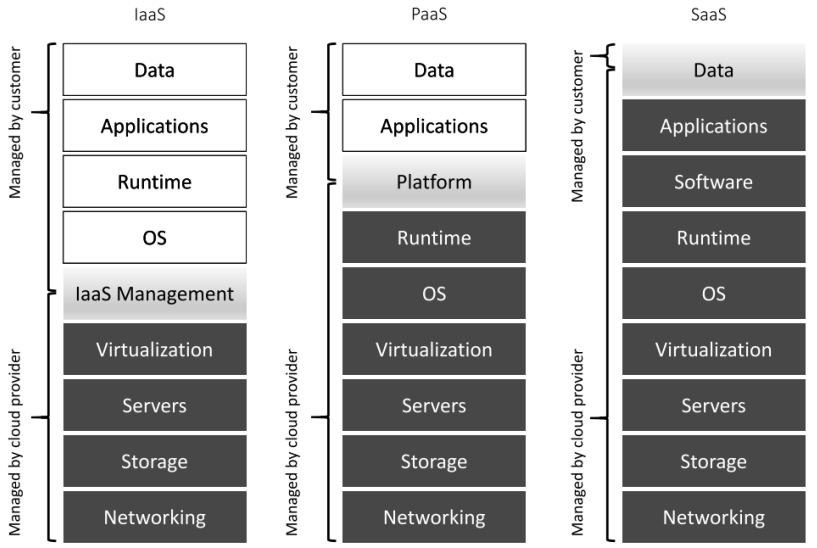
\includegraphics[scale=0.3]{imgs/cloud-services.png}
  \label{fig:cloud-services}
\end{figure} \\
Hiểu được những yêu cầu đó, các nhà cung cấp có những xuất bản riêng \cite{geewax2018google, wittig2018amazon} giúp người dùng dễ dàng hơn trong lựa chọn dịch vụ


% \bibliographystyle{plain} % We choose the "plain" reference style
% \bibliography{references} % Entries are in the refs.bib file
\printbibliography[heading=bibintoc, title = {TÀI LIỆU THAM KHẢO}]
\end{document}

